\documentclass{article}
\usepackage[english,russian]{babel}
\usepackage{textcomp}
\usepackage{geometry}
  \geometry{left=2cm}
  \geometry{right=1.5cm}
  \geometry{top=1.5cm}
  \geometry{bottom=2cm}
\usepackage{tikz}
\usepackage{multicol}
\usepackage{hyperref}
\usepackage{listings}
\usepackage{pmboxdraw}
\usepackage{fancyvrb}
\usepackage[shortlabels]{enumitem}
\pagenumbering{gobble}

\lstdefinestyle{csMiptCppStyle}{
  language=C++,
  basicstyle=\linespread{1.1}\ttfamily,
  columns=fixed,
  fontadjust=true,
  basewidth=0.5em,
  keywordstyle=\color{blue}\bfseries,
  commentstyle=\color{gray},
  texcl=true,
  stringstyle=\ttfamily\color{orange!50!black},
  showstringspaces=false,
  numbersep=5pt,
  numberstyle=\tiny\color{black},
  numberfirstline=true,
  stepnumber=1,      
  numbersep=10pt,
  backgroundcolor=\color{white},
  showstringspaces=false,
  captionpos=b,
  breaklines=true
  breakatwhitespace=true,
  xleftmargin=.2in,
  extendedchars=\true,
  keepspaces = true,
  tabsize=4,
  upquote=true,
}


\lstdefinestyle{csMiptCppLinesStyle}{
  style=csMiptCppStyle,
  frame=lines,
}

\lstdefinestyle{csMiptCppBorderStyle}{
  style=csMiptCppStyle,
  framexleftmargin=5mm, 
  frame=shadowbox, 
  rulesepcolor=\color{gray}
}


\lstdefinestyle{csMiptBash}{
  	style=csMiptCppStyle,
	breaklines=true,
	frame=tb,
	language=bash,
	breakatwhitespace=true,
	alsoletter={*()"'0123456789.},
	alsoother={\{\=\}},
	basicstyle={\ttfamily},
	keywordstyle={\bfseries},
	literate={{=}{{{=}}}1},
	prebreak={\textbackslash},
	sensitive=true,
	stepnumber=1,
	tabsize=4,
	morekeywords={echo, function},
	otherkeywords={-, \{, \}},
	literate={\$\{}{{{{\bfseries{}\$\{}}}}2,
	upquote=true,
	frame=none
}

\lstset{style=csMiptBash}
\lstset{
        literate={~}{{\raisebox{0.5ex}{\texttildelow}}}{1}
}


\renewcommand{\thesubsection}{\arabic{subsection}}
\makeatletter
\def\@seccntformat#1{\@ifundefined{#1@cntformat}%
   {\csname the#1\endcsname\quad}
   {\csname #1@cntformat\endcsname}}
\newcommand\section@cntformat{}     
\newcommand\subsection@cntformat{Задача \thesubsection.\space} 
\newcommand\subsubsection@cntformat{\thesubsubsection.\space}
\makeatother



\begin{document}
\title{Семинар \#2: git, продолжение. Практика. \vspace{-5ex}}\date{}\maketitle

\subsection*{Как сдавать задачи}
Для сдачи ДЗ вам нужно создать репозиторий на GitLab (если он ещё не создан) под названием \texttt{devtools-homework}. Структура репозитория должна иметь вид:
\begin{center}
\begin{BVerbatim}
├── seminar1_git/
│   ├── ...
├── seminar2_more_git/
│   ├── 01.txt
│   ├── 02.sh
│   └── ...
└── ...
\end{BVerbatim}
\end{center}
Для каждой задачи, если не сказано иное, необходимо создать bash-скрипт, содержащий решение, и отправить его в ваш репозиторий. Название скрипта должно соответствовать номеру задачи (например \texttt{02.sh} или \texttt{05a.sh}). 

\subsubsection*{Как сдавать задачи с интерактивным перебазированием}
Если в задаче используется интерактивное перебазирование, то помимо скрипта вам нужно будет отправить файл \texttt{git-rebase-todo} (после сделанных вами изменений). Название этого файла тоже должно начинаться с номера задачи, например \texttt{05b-git-rebase-todo.txt}.
Например, для решения задачи 5b вам надо отправить:
\begin{itemize}
\item Файл \texttt{05b.sh}, содержащий строки:
\begin{lstlisting}
#!/bin/bash
git rebase -i HEAD~4
\end{lstlisting}
\item Файл \texttt{05b-git-rebase-todo.txt}, содержащий строки:
\begin{lstlisting}
pick 6093969 CD: add dog.txt
pick 5804b31 CC: add cat.txt
pick 47a3a85 CB: add bat.txt
pick 7e06a13 CA: add axolotl.txt
\end{lstlisting}
\end{itemize}

\vspace{-3mm}
\subsection*{Подготовка. Генерация репозитория, который будет использоваться в задачах.}

Для решения некоторых задач вам потребуется создать простой репозиторий, состоящий из четырёх коммитов, с помощью bash-скрипта. Для этого сделайте следующее:

\begin{minipage}{0.65\linewidth}
\begin{enumerate}
\item Зайдите в репозиторий \href{https://mipt-hsse.gitlab.yandexcloud.net/v.biryukov/devtools_course}{\texttt{v.biryukov/devtools\_course}}, пройдите в папку
\texttt{seminar2\_more\_git/practice}, откройте файл \texttt{create\_animals.sh} и скачайте его.

\item Скопируйте скрипт в папку для запуска. Убедитесь, что эта папка не является частью другого репозитория и не содержит папку \texttt{animals}.


\item Откройте терминал. Зайдите в папку для запуска, добавьте скрипту права на исполнение и запустите его. Используйте команды:
\begin{lstlisting}
$ cd имяпапки
$ chmod +x create_animals.sh
$ ./create_animals.sh
\end{lstlisting}

\item Перейдите в папку \texttt{animals} и убедитесь, что репозиторий создался корректно, напечатав дерево коммитов:
\begin{lstlisting}[style=csMiptBash]
$ cd animals
$ git log --oneline --graph --all
\end{lstlisting}
\end{enumerate}
\end{minipage}
\hspace{1cm}
\begin{minipage}{0.3\linewidth}
\begin{center}
\includegraphics[scale=0.75]{../images/animals.png}
\end{center}
\end{minipage}


\newpage
\subsection{Способы адресации коммитов}
\definecolor{hashcolor}{RGB}{193, 156, 0}
\definecolor{headcolor}{RGB}{85, 214, 214}
\definecolor{branchcolor}{RGB}{22, 198, 12}

Пусть граф коммитов выглядит так, как это изображено на рисунке:
\begin{center}
\includegraphics[scale=0.8]{../images/graph_with_merges.png}
\end{center}
Коммит \texttt{C4} -- это коммит слияния ветки \texttt{featureA} в ветку \texttt{main}, а \texttt{C7} -- это коммит слияния \texttt{featureB} в \texttt{main}. \\
После этого вызвали команду \texttt{git log} вот так:
\begin{lstlisting}[style=csMiptBash,escapeinside={<@}{@>}]
$ git log --oneline --all --graph
*  <@\textcolor{hashcolor}{cc17ea1}@> (<@\textcolor{headcolor}{HEAD}@> -> <@\textcolor{branchcolor}{main}@>) C7
|\
| * <@\textcolor{hashcolor}{9e18dac}@> (<@\textcolor{branchcolor}{featureB}@>) C6
| * <@\textcolor{hashcolor}{eace0bf}@> C3
* | <@\textcolor{hashcolor}{00d7b4b}@> C5
* |   <@\textcolor{hashcolor}{38d17da}@> C4
|\ \
| |/
|/|
| * <@\textcolor{hashcolor}{4ed9ec3}@> (<@\textcolor{branchcolor}{featureA}@>) C2
* | <@\textcolor{hashcolor}{3599341}@> C1
|/
* <@\textcolor{hashcolor}{7afecc8}@> C0
\end{lstlisting}
Для каждого пункта ниже напишите команду или выражение, которое идентифицирует указанный коммит.
\begin{enumerate}
\item Хэш-адрес коммита \texttt{C0}
\item Адрес коммита \texttt{C0}, используя символы относительной адресации (\texttt{$\sim$} и \texttt{\textsuperscript{$\wedge$}}) от текущего положения \texttt{HEAD}.
\item Адрес коммита \texttt{C0}, используя относительную адресацию от указателя ветки \texttt{main}.
\item Хэш-адрес коммита \texttt{C3}
\item Адрес коммита \texttt{C3}, используя относительную адресацию от указателя ветки \texttt{featureB}.
\item Адрес коммита \texttt{C3}, используя относительную адресацию от указателя \texttt{HEAD}.
\item Хэш-адрес коммита \texttt{C2}
\item Адрес коммита \texttt{C2}, используя относительную адресацию от указателя ветки \texttt{featureA}.
\item Адрес коммита \texttt{C2}, используя относительную адресацию от указателя \texttt{HEAD}.
\end{enumerate}
Для того чтобы сдать эту задачу, создайте файл \texttt{01.txt} со всеми ответами и отправьте его в ваш репозиторий для сдачи заданий.

\subsection{Отмена индексации}
Предположим, что вы создали новый файл и добавили его в область индексирования, используя команды:
\begin{lstlisting}[style=csMiptBash]
$ touch emu.txt
$ git add emu.txt
\end{lstlisting}
Однако, затем передумали и хотите убрать этот файл из области индексирования.
Выполните команду, которая бы убирала этот файл из области индексирования, но оставляла бы файл в рабочей папке. Добавлять новые коммиты в этой задаче нельзя.

\subsection{Отмена коммита}
Предположим, что вы создали новый файл и добавили его в область индексирования и в локальный репозиторий:
\begin{lstlisting}[style=csMiptBash]
$ touch emu.txt
$ git add emu.txt
$ git commit -m "CE: add emu.txt"
\end{lstlisting}
Однако, затем передумали и хотите отменить коммит. При этом вы хотите, чтобы файл \texttt{emu.txt} продолжал находиться и в рабочей папке и в области индексирования. Выполните команду, которая отменит коммит, оставив рабочую папку и область индексирования неизменными.

\subsection{Отмена \texttt{reset}}
Предположим, что вы решили удалить все коммиты, кроме первого и, находясь на коммите \texttt{CD} (\textit{add dog}), выполнили:
\begin{lstlisting}
$ git reset --hard HEAD~4
\end{lstlisting}
Но потом передумали, и решили вернуть всё обратно. Что для этого нужно сделать?\\
Для того, чтобы сдать эту задачу вам нужно создать текстовый файл \texttt{04.txt}, в котором нужно будет описать словами алгоритм действий для восстановления после \texttt{reset}.


\subsection{Обратить коммиты}
В этом задании вам нужно обратить коммиты как это показано на изображении. При этом создавать файлы вручную нельзя, можно только использовать команды \texttt{git}.
\begin{center}
\includegraphics[scale=0.8]{../images/reverse_animals.png}
\end{center}
Решите эту задачу двумя способами:
\begin{enumerate}[(a)]
\item Создав новую ветку на начальном коммите и добавляя коммиты с помощью \texttt{git cherry-pick}. После этого нужно будет удалить старую ветку и переименовать новую.
\item Используя интерактивное перебазирование.
\end{enumerate}

\subsection{Объединить коммиты}
Пересоздайте репозиторий с помощью скрипта \texttt{create\_animals.sh}.
В этом задании вам нужно объединить все коммиты в один как это показано на изображении. При этом создавать файлы вручную нельзя, можно только использовать команды \texttt{git}.
\begin{center}
\includegraphics[scale=0.8]{../images/squash_animals.png}
\end{center}
Решите эту задачу двумя способами:
\begin{enumerate}[(a)]
\item Используя \texttt{reset}.
\item Используя интерактивное перебазирование.
\end{enumerate}

\subsection{Удалить коммиты}
Пересоздайте репозиторий с помощью скрипта \texttt{create\_animals.sh}.
В этом задании вам нужно удалить два коммита, как это показано на изображении. При этом создавать или удалять файлы вручную нельзя, можно только использовать команды \texttt{git}.
\begin{center}
\includegraphics[scale=0.8]{../images/delete_commits_animals.png}
\end{center}
Решите эту задачу двумя способами:
\begin{enumerate}[(a)]
\item Используя \texttt{cherry-pick}.
\item Используя интерактивное перебазирование.
\end{enumerate}

\subsection{Перераспределить коммиты}
Пересоздайте репозиторий с помощью скрипта \texttt{create\_animals.sh}. В этом задании вам нужно перераспределить коммиты в новые ветки, как это показано на изображении. При этом создавать или удалять файлы вручную нельзя, можно только использовать команды \texttt{git}.
\begin{center}
\includegraphics[scale=0.8]{../images/rearrange_animals.png}
\end{center}


\subsection{Отмена слияния}
Создайте новый репозиторий с помощью скрипта \texttt{create\_branch\_animals.sh} (его можно скачать оттуда же, где находился предыдущий скрипт). В этом репозитории будет 2 ветки: \texttt{main} и \texttt{other}. Предположим, что вы сделали слияние с помощью команд:
\begin{lstlisting}[style=csMiptBash]
$ git switch main
$ git merge other -m "CM: merging"
\end{lstlisting}

\begin{center}
\includegraphics[scale=0.8]{../images/branch_animals_merge.png}
\end{center}

\noindent Однако потом передумали и хотите отменить слияние. Напишите команды \texttt{git}, которые бы отменяли слияние и возвращали бы всё как прежде.


\subsection{Отмена перебазирования}
Создайте новый репозиторий с помощью скрипта \texttt{create\_branch\_animals.sh}. В этом репозитории есть 2 ветки: \texttt{main} и \texttt{other}. Предположим, что вы сделали перебазирование ветки \texttt{other} на ветку \texttt{main} с помощью команд:
\begin{lstlisting}[style=csMiptBash]
$ git switch other
$ git rebase main
\end{lstlisting}

\begin{center}
\includegraphics[scale=0.8]{../images/branch_animals_rebase.png}
\end{center}

\noindent Однако потом передумали и хотите отменить перебазирование. Напишите команды \texttt{git}, которые бы отменяли перебазирование и возвращали бы всё как прежде.

\subsection{Отмена \texttt{push}}
Для этой задачи вам нужно:
\begin{enumerate}
\item Создать новый локальный репозиторий на вашем компьютере с помощью скрипта \texttt{create\_animals.sh}.
\item Создать новый пустой репозиторий на GitLab.
\item Скопировать ссылку на GitLab репозиторий (протокол SSH).
\item Добавить новый remote на вашем локальном репозитории. 
\begin{lstlisting}[style=csMiptBash]
$ git remote add имя ссылка
\end{lstlisting}
Имя можно выбрать любое, но часто выбирают \texttt{origin}.
\item Проверьте, что новый remote добавился:
\begin{lstlisting}[style=csMiptBash]
$ git remote -v
\end{lstlisting}
\item Отправьте ветки \texttt{main} и \texttt{other} вашего локального репозитория на удалённый репозиторий GitLab.
\begin{lstlisting}[style=csMiptBash]
$ git push -u origin main other
\end{lstlisting}
\end{enumerate}

\noindent Предположим, что вы создали новый файл и добавили его в область индексирования, в локальный репозиторий, а затем и в удалённый репозиторий.
\begin{lstlisting}[style=csMiptBash]
$ touch emu.txt
$ git add emu.txt
$ git commit -m "CE: add emu.txt"
$ git push
\end{lstlisting}
Однако затем передумали и хотите отменить коммит. Вы хотите, чтобы изменения пропали везде -- как на вашем компьютере, так и в последнем состоянии удалённого репозитория. Решите эту задачу двумя способами:
\begin{itemize}
\item Используя \texttt{git push}.
\item Используя \texttt{git revert}.
\end{itemize}



\subsection{Игнорирование}
Вы работаете над проектом на языке C и используете Git для контроля версий. В процессе разработки, компиляции и работы в разных средах создаются файлы, которые не должны попадать в репозиторий. А именно, в репозиторий не должно попадать следующее:

\begin{itemize}
\item \textbf{Логи проекта}\\
Папки с названием \texttt{logs}, в какой бы директории проекта они не находились.

\item \textbf{Служебные файлы операционных систем}\\
Файлы с названиями \texttt{Thumbs.db} и \texttt{.DS\_Store}, в какой бы директории проекта они не находились. Это скрытые служебные файлы, которые генерируются операционными системами Windows и macOS соответственно.

\item \textbf{Файлы IDE}\\
Папки с названием \texttt{.vscode} и \texttt{.idea}, в какой бы директории проекта они не находились. Эти папки генерируются при использовании IDE Visual Studio и IDE от JetBrains соответственно.

\item \textbf{Файлы, создаваемые при компиляции}\\
Любые файлы с расширениями \texttt{.exe}, \texttt{.a}, \texttt{.lib} \texttt{.dll}, \texttt{.o}, \texttt{.so}, в какой бы директории они не находились.

\item \textbf{Папка сборки}\\
Папка \texttt{build} в корневой директории проекта. Но в поддиректориях папка с таким названием игнорироваться не должна.

\item \textbf{Конфигурационные файлы}\\
Файлы с расширением \texttt{.cfg}, в какой бы директории проекта они не находились. За исключением файла \texttt{config/settings.cfg}, который не должен игнорироваться.
\end{itemize}
Напишите файл \texttt{.gitignore} для такого проекта. Протестируйте этот файл на одном из созданных ранее репозиториев.
Для сдачи этого задания поместите файл \texttt{.gitignore} в ваш репозиторий для сдачи заданий.


\subsection{Форк}
Зайдите на GitLab и сделайте форк репозитория \href{https://mipt-hsse.gitlab.yandexcloud.net/v.biryukov/branch_animals}{mipt-hsse.gitlab.yandexcloud.net/v.biryukov/branch\_animals}. Клонируйте форк на свой компьютер. Создайте новую ветку на коммите \texttt{HEAD}. Добавьте в этой ветке новый коммит, содержащий файл с новым животным (на ваш выбор). Отправьте изменения на ваш форк. Сделайте merge request, чтобы добавить изменения в изначальный репозиторий (\texttt{v.biryukov/branch\_animals}).

\noindent Для сдачи этого задания убедитесь, что ваш форк является публичным.


\subsection{Тэги}
Создайте 2 новых тэга в репозитории \texttt{branch\_animals}: один на коммите \texttt{CA} -- \texttt{v0.0.1}, второй на коммите \texttt{CD} -- \texttt{v0.1.0}. Проверьте, что тэги созданы:
\begin{lstlisting}
git log --oneline --graph --all
\end{lstlisting}
Для сдачи этого задания отправьте теги на удалённый сервер на GitLab.



\iffalse
\subsection{Pre-commit hook}
Напишите pre-commit хук, который будет проверять, что все файлы имеют расширение \texttt{.txt}. Проверьте работу этого хука, закоммитив файл с другим расширением.
\fi


\end{document}
